\documentclass[10pt,twocolumn]{article}

\usepackage[utf8]{inputenc}
\usepackage[T1]{fontenc}
\usepackage{times}
\usepackage{microtype}
\usepackage[
    letterpaper,
    margin=0.72in,
    columnsep=0.24in
]{geometry}
\usepackage{amsmath}
\usepackage{amssymb}
\usepackage{mathtools}
\usepackage{graphicx}
\usepackage{booktabs}
\usepackage{multirow}
\usepackage{array}
\usepackage{tabularx}
\usepackage{makecell}
\usepackage{caption}
\usepackage{subcaption}
\usepackage[numbers,sort&compress]{natbib}
\usepackage[hidelinks]{hyperref}
\usepackage{xcolor}
\usepackage{enumitem}
\usepackage{titlesec}
\usepackage{placeins}
\usepackage{float}
\usepackage{dblfloatfix}
\usepackage{balance}

\setlist{nosep,leftmargin=*}
\titlespacing*{\section}{0pt}{0.85em}{0.45em}
\titlespacing*{\subsection}{0pt}{0.65em}{0.35em}
\titlespacing*{\subsubsection}{0pt}{0.5em}{0.25em}
\captionsetup{
    font=small,
    labelfont=bf,
    justification=raggedright,
    singlelinecheck=false,
    skip=4pt
}
\setlength{\textfloatsep}{8pt plus 1pt minus 2pt}
\setlength{\floatsep}{6pt plus 1pt minus 2pt}
\setlength{\intextsep}{6pt plus 1pt minus 2pt}
\graphicspath{{../figures/}{figures/}}
% Favor dense two-column pages and flexible float placement.
\flushbottom
\setcounter{topnumber}{5}
\setcounter{bottomnumber}{5}
\setcounter{totalnumber}{10}
\setcounter{dbltopnumber}{4}
\renewcommand{\topfraction}{0.96}
\renewcommand{\bottomfraction}{0.96}
\renewcommand{\textfraction}{0.02}
\renewcommand{\floatpagefraction}{0.78}
\renewcommand{\dbltopfraction}{0.96}
\renewcommand{\dblfloatpagefraction}{0.78}
\setlength{\bibsep}{0pt}
\renewcommand{\bibfont}{\scriptsize}
\newcolumntype{Y}{>{\raggedright\arraybackslash}X}
\newcolumntype{Z}{>{\centering\arraybackslash}p{0.072\textwidth}}

\newcommand{\methodname}{Budget-Aware Early Exiting}
\newcommand{\dataset}{CIFAR-10}
\newcommand{\backbone}{ResNet-18}

\title{\vspace{-1.0em}
Learning When to Stop: Budget-Aware Early Exiting for Energy-Efficient CNN Inference
\vspace{-0.4em}
}

\author{
Tran Anh Chuong\\
VinUniversity\\
COMP2050 -- Artificial Intelligence Programming Project\\
\texttt{24chuong.ta@vinuni.edu.vn}
}

\date{}

\begin{document}

\twocolumn[
\maketitle

\begin{abstract}
This project studies adaptive early exiting for image classification on \dataset{} using a \backbone{} backbone with three intermediate classifiers and a final exit. The evaluation compares a full baseline, the jointly trained early-exit backbone, fixed-threshold routing, dynamic-threshold routing, a supervised learned controller, and a REINFORCE controller. In the source-of-truth run, the full baseline reaches 88.26\% test accuracy, while the early-exit backbone reaches 87.74\% when always using the final head. The strongest fixed-threshold result preserves 87.73\% accuracy at 32.83\% floating-point operations (FLOPs) reduction with threshold $\tau = 0.99$, and the strongest REINFORCE run preserves 87.69\% accuracy at 49.54\% FLOPs reduction with $\lambda_{\text{cost}} = 0.05$. By contrast, the best-accuracy dynamic-threshold configuration collapses to the final exit and yields no FLOPs savings, and the supervised best\_reward controller is overly aggressive, dropping to 72.52\% accuracy despite 74.33\% FLOPs reduction. These results suggest that simple high-confidence thresholding remains a strong baseline, while REINFORCE provides the best learned-policy tradeoff in the current CIFAR-10 study. Policy CO$_2$ values are reported as FLOPs-scaled estimates rather than direct emissions measurements.
\end{abstract}

\vspace{0.8em}
]

\section{Introduction}

Green AI argues that model quality should be evaluated together with computational cost, which makes inference efficiency an important part of responsible model design \cite{schwartz2019green}. In image classification, strong backbones such as residual networks deliver high accuracy, but standard deployment still applies the same full forward pass to every input regardless of difficulty \cite{he2015deep}. Compression and efficient-inference work has reduced deployment cost in many settings, yet much of that line of work still relies on one fixed computational budget for all examples \cite{han2015deep,han2021dynamic}.

Early-exit architectures offer a more input-dependent alternative. Instead of sending every image through the deepest layers, they attach intermediate classifiers so that easy examples can stop early while harder ones continue \cite{teerapittayanon2017branchynet,huang2017multiscale}. This idea is closely related to selective prediction, where confidence or risk estimates determine whether a model should commit to a decision under limited computation or uncertainty \cite{geifman2017selective}. More broadly, adaptive-computation methods frame the same question as a decision about how much computation each example deserves \cite{graves2016adaptive}.

This project asks whether adaptive exit policies can improve the accuracy-efficiency tradeoff of a \backbone{} classifier on \dataset{}. The comparison is intentionally broad: it includes a full baseline, the early-exit backbone without routing, fixed confidence thresholds, dynamic threshold schedules, a supervised exit controller, and a REINFORCE controller. The deeper experiment run dated 2026-06-20 is treated as the numeric source of truth throughout the paper.

The main contributions are:
\begin{itemize}
    \item an early-exit \backbone{} with exits after layers 1, 2, 3, and the final classifier;
    \item a unified empirical comparison of fixed-threshold, dynamic-threshold, supervised-controller, and REINFORCE policies on \dataset{};
    \item evaluation of accuracy, floating-point operations (FLOPs), latency, average exit depth, macro-F1, bootstrap confidence intervals, and estimated CO$_2$ impact;
    \item a careful discussion of where adaptive inference succeeds, where it collapses, and which measurements remain estimated rather than directly observed.
\end{itemize}

\section{Related Work}

Efficient neural inference has been studied through both static and dynamic methods. Static approaches such as Deep Compression reduce model cost by pruning, quantization, and coding, yielding smaller and cheaper networks without changing the compute path per input \cite{han2015deep}. Dynamic-neural-network work instead focuses on conditional execution, routing, or adaptive subnetworks that vary computation based on the current example, and recent surveys frame this as a broad family of input-adaptive models \cite{han2021dynamic}. The adaptive-computation perspective itself is older and appears clearly in Adaptive Computation Time, which formalizes the idea that different inputs may need different amounts of processing \cite{graves2016adaptive}.

Early-exit networks are one concrete adaptive strategy. BranchyNet showed that side branches can reduce latency and energy by allowing confident examples to terminate early, while MSDNet extended the idea to resource-efficient classification under both anytime and budgeted settings \cite{teerapittayanon2017branchynet,huang2017multiscale}. Confidence-based routing is attractive because it is simple and cheap, but it is also closely tied to the broader selective-classification problem, where the system must decide when it is reliable enough to act \cite{geifman2017selective}. This connection is relevant here because fixed and dynamic threshold policies ultimately depend on the quality of those confidence signals.

Learned routing policies provide a more flexible alternative to thresholding. SkipNet learns dynamic routing in convolutional networks with a hybrid supervised and reinforcement-learning procedure, while BlockDrop learns inference paths in residual networks with reinforcement learning over residual blocks \cite{wang2017skipnet,wu2017blockdrop}. These papers motivate the controller side of the present project: once routing is treated as a sequential decision problem, policy-gradient training becomes a natural tool for balancing prediction quality against compute cost. At the same time, the literature also suggests that learned routing can be sensitive to reward shaping and optimization details, so the present work treats supervised and REINFORCE controllers as empirical alternatives to strong threshold baselines rather than assuming they will dominate them automatically.

\section{Methodology}

\subsection{Baseline Model}

The reference model is a full \backbone{} classifier trained on \dataset{}. It performs the complete forward pass for every image and serves as the baseline for accuracy, FLOPs, latency, and the reference CO$_2$ metric recorded during training.

\subsection{Early-Exit Architecture}

The early-exit model reuses the CIFAR-style \backbone{} backbone and adds auxiliary classifiers after layers 1, 2, and 3, plus the final layer-4 classifier. The four exits are named `exit\_1', `exit\_2', `exit\_3', and `final\_exit'. The verified FLOPs ratios for these exits are 0.22, 0.42, 0.68, and 1.00, respectively.

For exit $i$, the probability vector is
\begin{equation}
    p_i = \operatorname{softmax}(z_i),
\end{equation}
where $z_i$ is the logit vector at exit $i$. The confidence score is
\begin{equation}
    c_i = \max_j p_i(j).
\end{equation}

The backbone is trained jointly across exits using a weighted sum of cross-entropy losses:
\begin{equation}
    \mathcal{L} = \sum_{i=1}^{K} \alpha_i \mathcal{L}_i,
\end{equation}
with verified loss weights $[\alpha_1, \alpha_2, \alpha_3, \alpha_4] = [0.3, 0.5, 0.7, 1.0]$. This training objective encourages earlier exits to become useful without discarding the deepest classifier.

Figure~\ref{fig:method-pipeline} summarizes the architectural difference between the full baseline and the early-exit backbone.

\begin{figure*}[!tbp]
    \centering
    \includegraphics[width=0.92\textwidth]{figure1Off.png}
    % \fbox{%
    % \begin{minipage}[c][0.24\textheight][c]{0.92\textwidth}
    %     \centering
    %     \textbf{Placeholder: Full Baseline vs. Early-Exit Backbone}\\[0.5em]
    %     \footnotesize
    %     Draw a two-lane left-to-right schematic. Top lane: CIFAR-10 image $\rightarrow$ full ResNet-18 backbone $\rightarrow$ final classifier $\rightarrow$ prediction. Bottom lane: CIFAR-10 image $\rightarrow$ stem/layer 1 + \texttt{exit\_1} (0.22x FLOPs) $\rightarrow$ layer 2 + \texttt{exit\_2} (0.42x) $\rightarrow$ layer 3 + \texttt{exit\_3} (0.68x) $\rightarrow$ layer 4 + \texttt{final\_exit} (1.00x). Add small decision markers after exits 1--3 labeled confidence or controller decision. Use distinct colors for backbone blocks, exit heads, and policy decisions; arrows should make clear that early-exit policies can stop before deeper layers.
    % \end{minipage}}
    \caption{Baseline and early-exit inference pipeline. The full \backbone{} baseline always executes the complete network, whereas the early-exit model exposes intermediate classifiers that allow fixed-threshold, dynamic-threshold, supervised-controller, and REINFORCE policies to stop computation early.}
    \label{fig:method-pipeline}
\end{figure*}

\subsection{Fixed Confidence Thresholding}

The fixed-threshold policy exits at the first head whose confidence exceeds a constant threshold $\tau$:
\begin{equation}
    \text{exit at } i \quad \text{if} \quad c_i \geq \tau.
\end{equation}
The deeper ablation run evaluates a dense sweep from $\tau = 0.50$ to $\tau = 0.99$ and therefore exposes the full tradeoff curve rather than only a small set of hand-picked thresholds.

Figure~\ref{fig:fixed-routing} shows the fixed-threshold decision rule at a single exit.

\begin{figure}[!tbp]
    \centering
    \includegraphics[width=0.94\linewidth]{figure2_confidence_based_threshold_routing.pdf}
    % \fbox{%
    % \begin{minipage}[c][0.18\textheight][c]{0.94\linewidth}
    %     \centering
    %     \textbf{Placeholder: Confidence-Based Threshold Routing}\\[0.5em]
    %     \footnotesize
    %     Draw a compact flowchart: exit logits $z_i$ $\rightarrow$ softmax probabilities $p_i$ $\rightarrow$ confidence $c_i=\max_j p_i(j)$ $\rightarrow$ compare $c_i \geq \tau$. Branch outcomes: yes $\rightarrow$ exit and predict; no $\rightarrow$ continue to the next block. Include a tiny example path where exit 1 has $c_1 < \tau$ and continues, while exit 2 has $c_2 \geq \tau$ and stops.
    % \end{minipage}}
    \caption{Fixed confidence-threshold routing at one exit. Each intermediate classifier produces a confidence score, and the policy stops at the first exit whose confidence exceeds the threshold $\tau$.}
    \label{fig:fixed-routing}
\end{figure}

\subsection{Budget-Aware Dynamic Thresholding}

Dynamic thresholding modifies the exit condition using the cumulative compute already consumed. Let
\begin{equation}
    r_i =
    \frac{\operatorname{FLOPs}_i}
    {\operatorname{FLOPs}_{\text{full}}}
\end{equation}
denote the normalized compute ratio at exit $i$. The term $\tau_{\text{base}}$ is the base confidence threshold: it is the starting threshold before any depth-dependent adjustment is applied, and therefore plays the same role as a fixed threshold when $\alpha = 0$. In the implementation, the accuracy-first mode increases the threshold with depth,
\begin{equation}
    \tau_i = \tau_{\text{base}} + \alpha r_i,
\end{equation}
while the budget-first mode decreases it with depth,
\begin{equation}
    \tau_i = \tau_{\text{base}} - \alpha r_i.
\end{equation}
This gives the policy extra flexibility, but it also introduces a second tuning parameter $\alpha$ and a design choice between accuracy-first and budget-first behavior.

Figure~\ref{fig:dynamic-schedule} contrasts the two dynamic threshold schedules.

\begin{figure}[!tbp]
    \centering
    \includegraphics[width=0.94\linewidth]{figure_threshold.png}
    % \fbox{%
    % \begin{minipage}[c][0.18\textheight][c]{0.94\linewidth}
    %     \centering
    %     \textbf{Placeholder: Dynamic Threshold Schedule}\\[0.5em]
    %     \footnotesize
    %     Draw a small conceptual plot with exit depth or FLOPs ratio $r_i$ on the x-axis and threshold $\tau_i$ on the y-axis. Show a horizontal reference line for $\tau_{\text{base}}$. Add an upward line for accuracy-first, labeled $\tau_i=\tau_{\text{base}}+\alpha r_i$, and a downward line for budget-first, labeled $\tau_i=\tau_{\text{base}}-\alpha r_i$. Annotate that $\alpha=0$ collapses the policy back to a fixed threshold.
    % \end{minipage}}
    \caption{Dynamic threshold schedules. The base threshold $\tau_{\text{base}}$ sets the starting confidence requirement, while $\alpha$ adjusts how strict or permissive the policy becomes as more computation has already been spent.}
    \label{fig:dynamic-schedule}
\end{figure}

\subsection{Supervised Exit Controller}

The supervised controller is a small multilayer perceptron trained as a stage-wise binary decision rule rather than a 4-way exit classifier. At each non-final exit it predicts whether the model should \emph{continue} or \emph{exit now}. For the supervised path, the feature vector used by the implementation is
\begin{equation}
    s_i^{\text{sup}} = [c_i, H_i, m_i, e_i, r_i],
\end{equation}
where $H_i$ is entropy, $m_i$ is the top-1/top-2 margin, $e_i$ is the raw exit index, and $r_i$ is the FLOPs ratio. Entropy and margin are computed as
\begin{equation}
    H_i = -\sum_j p_i(j)\log p_i(j),
\end{equation}
\begin{equation}
    m_i = p_i(\text{top-1}) - p_i(\text{top-2}).
\end{equation}

This controller is supervised because its targets are generated offline from a frozen early-exit backbone and then learned with standard cross-entropy. The implementation first chooses one target exit per sample. Under \texttt{earliest\_correct}, the target is the first exit whose prediction matches the ground-truth label; if no early exit is correct, the target defaults to the final exit. Under \texttt{best\_reward}, the target is the exit that maximizes
\begin{equation}
    \mathbf{1}[\hat{y}_i = y] - \lambda r_i,
\end{equation}
so changing $\lambda$ changes the supervision target itself. After the target exit is chosen, the dataset builder creates one training example for each non-final exit up to that target: the label is $1$ if the current exit is the selected target exit and $0$ if the controller should continue deeper. Exits after the chosen target are dropped from the supervised dataset because the routing decision has already been resolved. The deeper controller sweep reported later uses \texttt{best\_reward} supervision rather than the earlier \texttt{earliest\_correct} baseline, which makes the lambda sweep a genuine reward-label ablation instead of a purely optimization-side hyperparameter search.

Figure~\ref{fig:supervised-labels} illustrates how generated target exits become supervised binary decisions.

\begin{figure*}[!tbp]
    \centering
    \includegraphics[width=0.92\textwidth]{figure4.png}
    % \fbox{%
    % \begin{minipage}[c][0.24\textheight][c]{0.90\textwidth}
    %     \centering
    %     \textbf{Placeholder: Supervised Controller Label Generation}\\[0.5em]
    %     \footnotesize
    %     Draw a pipeline from frozen early-exit backbone $\rightarrow$ all exit logits and predictions $\rightarrow$ label generator $\rightarrow$ stage-wise controller dataset $\rightarrow$ MLP trained with cross-entropy. In the label generator, show two options: \texttt{earliest\_correct} selects the first correct exit, and \texttt{best\_reward} selects $\arg\max_i\,\mathbf{1}[\hat{y}_i=y]-\lambda r_i$. In the dataset-builder block, show records for exits before or at the target: \texttt{continue = 0} until the selected target exit, then \texttt{exit now = 1}. Use a callout that exits after the target are not included.
    % \end{minipage}}
    \caption{Supervised controller training pipeline. The controller is supervised because the frozen early-exit model first generates target exits, which are converted into binary continue-or-exit labels for stage-wise cross-entropy training.}
    \label{fig:supervised-labels}
\end{figure*}

\subsection{REINFORCE Exit Controller}

The REINFORCE controller reuses the same MLP layout, but replaces offline imitation targets with online policy optimization over sequential routing decisions. At each non-final exit it defines a stochastic policy
\begin{equation}
    \pi_\theta(a_i \mid s_i),
\end{equation}
where $a_i \in \{\text{continue}, \text{exit}\}$. The policy reward is
\begin{equation}
    R =
    \mathbf{1}\{\hat{y}=y\}
    -
    \lambda_{\text{cost}} r_i.
\end{equation}
In the reported run, the optional wrong-prediction penalty available in code is inactive because \texttt{wrong\_penalty} is set to $0.0$. The RL state uses the normalized variant implemented for REINFORCE,
\begin{equation}
    s_i^{\text{rl}} = [c_i, \tilde{H}_i, m_i, d_i, r_i],
\end{equation}
where $\tilde{H}_i = H_i / \log C$ is entropy normalized by the number of classes and $d_i$ is normalized exit depth. During training, the policy samples an action at each non-final exit; if it never selects \emph{exit}, the sample is forced to the final classifier.

The objective is to maximize expected reward,
\begin{equation}
    J(\theta) = \mathbb{E}_{\pi_\theta}[R],
\end{equation}
which the implementation optimizes in loss form as
\begin{equation}
    \mathcal{L}_{\text{pg}}
    =
    -(R - b)\sum_t \log \pi_\theta(a_t \mid s_t)
    -
    \beta \sum_t H\!\left(\pi_\theta(\cdot \mid s_t)\right),
\end{equation}
where $b$ is a moving-average reward baseline and $\beta$ is the entropy-regularization weight. The baseline is updated after each batch as
\begin{equation}
    b \leftarrow \mu b + (1-\mu)\bar{R}_{\text{batch}}.
\end{equation}
The implementation freezes the early-exit backbone during policy optimization, warm-starts the controller from a supervised checkpoint by default, clips gradients to stabilize training, and selects the best checkpoint by validation average reward. At test time, evaluation is deterministic: the controller uses the argmax policy action at each exit rather than sampling. In short, the supervised controller imitates labels generated from backbone outputs, whereas REINFORCE directly optimizes expected reward over the sequential exit decisions themselves. The reported sweep varies $\lambda_{\text{cost}} \in \{0.05, 0.10, 0.20, 0.30, 0.50\}$.

Figure~\ref{fig:reinforce-policy} connects the sequential exit process to the REINFORCE update.

\begin{figure*}[!tbp]
    \centering
    \includegraphics[width=0.92\textwidth]{figure5.png}
    % \fbox{%
    % \begin{minipage}[c][0.26\textheight][c]{0.90\textwidth}
    %     \centering
    %     \textbf{Placeholder: REINFORCE Sequential Exit Policy}\\[0.5em]
    %     \footnotesize
    %     Draw a sequential decision diagram across \texttt{exit\_1}, \texttt{exit\_2}, \texttt{exit\_3}, and \texttt{final\_exit}. At exits 1--3, show state $s_i^{\text{rl}}$ entering the controller, a categorical action sampled during training, and branches for \texttt{continue} or \texttt{exit}. Add a forced-final-exit path when no earlier exit is selected. On the right, show reward computation $R=\mathbf{1}[\hat{y}=y]-\lambda_{\text{cost}}r_i$ and the policy-gradient loss with moving-average baseline $b$, entropy regularization $\beta$, and gradient clipping. Add a test-time callout: use argmax action rather than sampling.
    % \end{minipage}}
    \caption{REINFORCE controller training and evaluation flow. Unlike the supervised controller, the REINFORCE policy samples sequential routing actions during training and updates the controller from the reward assigned to the selected exit.}
    \label{fig:reinforce-policy}
\end{figure*}

\section{Experimental Setup}

\subsection{Dataset and Training Setup}

The study uses \dataset{}, a 10-class image classification benchmark \cite{krizhevsky2009cifar}. The verified data settings are a batch size of 128 and a validation split of 0.1. The baseline is trained for 20 epochs and the early-exit backbone for 25 epochs. Controller and REINFORCE runs use the trained early-exit checkpoint rather than retraining the backbone from scratch.

\subsection{Compared Methods}

The final comparison includes:
\begin{itemize}
    \item the full \backbone{} baseline;
    \item the early-exit \backbone{} evaluated at the final head only;
    \item the best-accuracy fixed-threshold policy from the dense threshold sweep;
    \item the best-accuracy dynamic-threshold policy from the dynamic sweep;
    \item the best-accuracy supervised \texttt{best\_reward} controller;
    \item the best-accuracy REINFORCE controller.
\end{itemize}

Because the run-specific \texttt{comparison.csv} only contains the baseline and early-exit rows, the representative policy-family rows in Table~\ref{tab:main-results} are taken from the \texttt{best\_result} entries of the family-specific JSON outputs.

\subsection{Evaluation Metrics}

The report uses accuracy, macro-F1, weighted-F1, FLOPs per sample, FLOPs reduction, latency per sample, average exit depth, exit distribution, and reward when applicable. FLOPs reduction is
\begin{equation}
    \operatorname{Reduction}
    =
    1 -
    \frac{\operatorname{FLOPs}_{\text{method}}}
    {\operatorname{FLOPs}_{\text{full}}}.
\end{equation}

Latency for threshold, dynamic-threshold, supervised-controller, and REINFORCE policies in the source-of-truth run is measured from staged conditional execution. By contrast, policy CO$_2$ values are not direct emissions measurements: they are FLOPs-scaled estimates derived from the baseline reference. The baseline and early-exit CO$_2$ values come from CodeCarbon-wrapped training runs, so the table reports a mixed efficiency record that must be interpreted cautiously.

\subsection{Statistical Analysis}

The project includes bootstrap resampling of deterministic test predictions, which provides mean, standard deviation, and 95\% confidence intervals without retraining new seeds. However, the current evidence does not establish multiple independent full training runs for every method. Following the experimental log, the results should therefore be interpreted as an empirical case study rather than a statistically conclusive benchmark.

\section{Results}

\subsection{Main Accuracy--Efficiency Tradeoff}

Table~\ref{tab:main-results} summarizes one representative result per method family. The fixed-threshold and REINFORCE rows are the strongest practical tradeoff points in the current evidence. Figure~\ref{fig:accuracy-flops} shows the broader frontier: fixed thresholds and REINFORCE dominate the supervised controller, while dynamic thresholding often overlaps with simpler fixed-threshold behavior or collapses to the final exit.

\begin{table*}[!tbp]
\centering
\caption{Main comparison across representative methods. Baseline and early-exit rows come from the run-specific \texttt{comparison.csv}; policy-family rows come from the \texttt{best\_result} entries of the family-specific JSON files. Baseline and early-exit CO$_2$ are CodeCarbon training-run values, while policy CO$_2$ values are FLOPs-scaled estimates.}
\label{tab:main-results}
\footnotesize
\setlength{\tabcolsep}{3pt}
\renewcommand{\arraystretch}{1.05}
\begin{tabularx}{\textwidth}{@{}Ycccccc@{}}
\toprule
Method & Accuracy & \makecell{FLOPs/\\sample} & \makecell{FLOPs\\Red.} & \makecell{Latency/\\sample} & \makecell{CO$_2$\\metric} & \makecell{Avg.\\Exit} \\
\midrule
Full \backbone{} & 88.26\% & 557.89M & 0.00\% & 2.182 ms & $9.23 \times 10^{-5}$ kg & Final \\
Early-exit \backbone{} & 87.74\% & 558.01M & 0.00\% & 2.606 ms & $1.49 \times 10^{-4}$ kg & N/A \\
Fixed threshold ($\tau=0.99$) & 87.73\% & 374.72M & 32.83\% & 0.080 ms & $6.20 \times 10^{-5}$ kg est. & 2.88 \\
Dynamic threshold (acc.-first, $0.90/0.50$) & 87.74\% & 557.89M & 0.00\% & 0.086 ms & $9.23 \times 10^{-5}$ kg est. & 4.00 \\
Supervised controller ($\lambda=0.30$) & 72.52\% & 143.22M & 74.33\% & 0.053 ms & $2.37 \times 10^{-5}$ kg est. & 1.18 \\
REINFORCE controller ($\lambda=0.05$) & 87.69\% & 281.52M & 49.54\% & 0.086 ms & $4.66 \times 10^{-5}$ kg est. & 2.32 \\
\bottomrule
\end{tabularx}
\end{table*}

\begin{figure*}[!tbp]
    \centering
    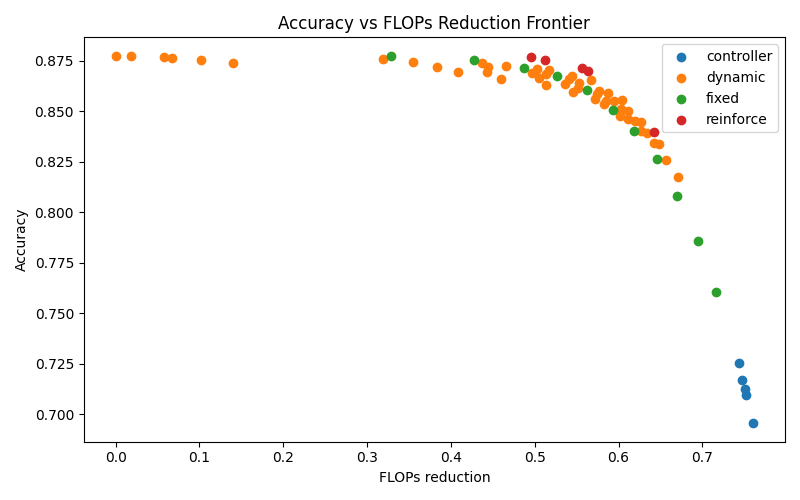
\includegraphics[width=0.94\textwidth,height=0.40\textheight,keepaspectratio]{accuracy_flops_frontier.png}
    \caption{Accuracy versus FLOPs reduction across all evaluated policy families in the deeper experiment run. Fixed thresholds and REINFORCE occupy the strongest tradeoff region, while the supervised \texttt{best\_reward} controller remains far below the main frontier.}
    \label{fig:accuracy-flops}
\end{figure*}

The full baseline reaches 88.26\% accuracy, and the early-exit backbone evaluated only at the final head reaches 87.74\%. This means the backbone modification itself causes only a modest 0.52-point accuracy gap relative to the full baseline, which makes the subsequent policy comparison meaningful.

Among hand-designed policies, the best fixed-threshold accuracy point is $\tau = 0.99$, with 87.73\% accuracy and 32.83\% FLOPs reduction. This result is only 0.01 points below the early-exit final head and 0.53 points below the full baseline, while still routing 64.14\% of test samples to an intermediate exit. The dynamic-threshold family performs less convincingly in the source-of-truth run: the best-accuracy configuration is the accuracy-first policy with base threshold 0.90 and $\alpha = 0.50$, but it exits every sample at the final head and therefore achieves 0\% FLOPs reduction. In other words, dynamic thresholding does not beat the simpler fixed-threshold baseline in this run.

Figure~\ref{fig:threshold-ablation} shows a smooth threshold tradeoff. Lower thresholds exit very aggressively, while higher thresholds preserve accuracy by leaving more hard examples for deeper heads. The fixed-threshold sweep therefore provides a strong and interpretable control curve for every learned policy.

The learned-policy picture is more mixed. The supervised \texttt{best\_reward} controller reaches its best accuracy at $\lambda = 0.30$, but that still yields only 72.52\% accuracy even though it saves 74.33\% of FLOPs on average. Its exit distribution reveals the cause: 82.63\% of samples terminate at the first exit, and the controller never uses the final head in the selected best-accuracy run. This is a clear over-exiting failure mode.

REINFORCE behaves much better. The best-accuracy REINFORCE run uses $\lambda_{\text{cost}} = 0.05$ and reaches 87.69\% accuracy with 49.54\% FLOPs reduction. Its exit distribution is more balanced than the supervised controller's: 68.93\% of samples leave at exit 2, 29.87\% at exit 3, and only 1.20\% proceed to the final head. This learned policy is the strongest controller result in the current evidence, but it still trails the strongest fixed-threshold policy slightly in accuracy.

For easier side-by-side reading, the three policy-sweep plots are grouped together in Figure~\ref{fig:policy-sweeps} beneath the main two-column frontier figure.

\begin{figure*}[!tbp]
    \centering
    \begin{subfigure}[t]{0.32\textwidth}
        \centering
        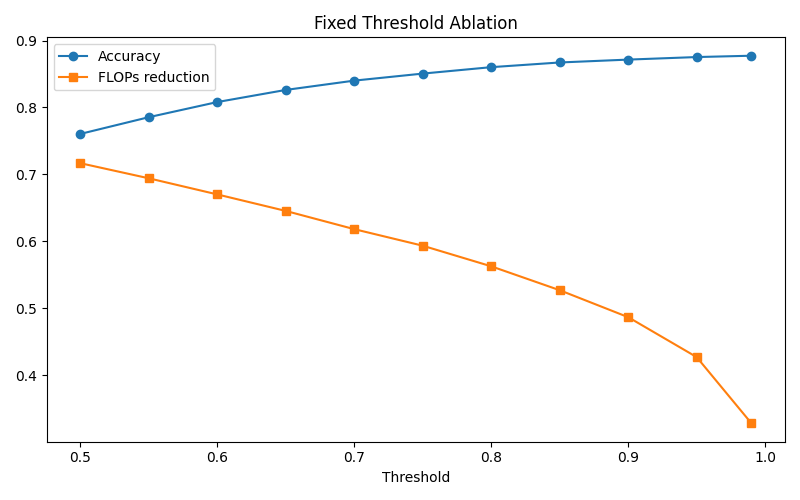
\includegraphics[width=\linewidth,height=0.145\textheight,keepaspectratio]{accuracy_vs_threshold.png}
        \caption{Fixed-threshold ablation. Higher confidence thresholds improve accuracy but reduce the amount of computation saved.}
        \label{fig:threshold-ablation}
    \end{subfigure}\hfill
    \begin{subfigure}[t]{0.32\textwidth}
        \centering
        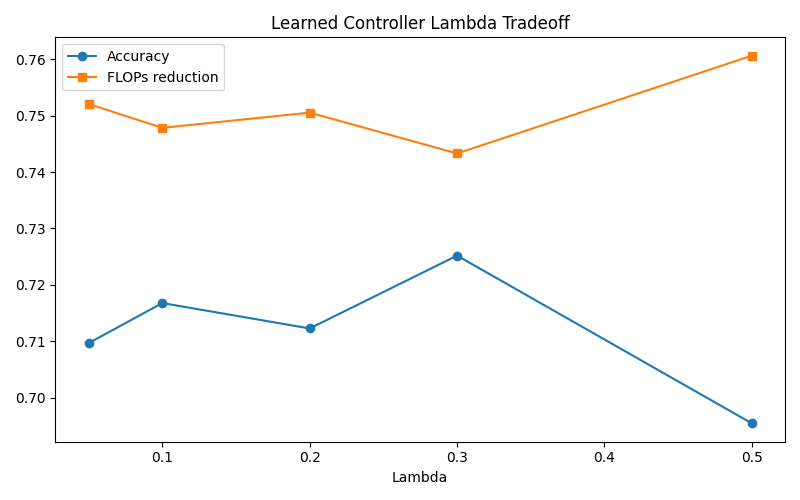
\includegraphics[width=\linewidth,height=0.145\textheight,keepaspectratio]{controller_lambda_tradeoff.png}
        \caption{Supervised \texttt{best\_reward} controller sweep. Every setting remains far below the strongest threshold and REINFORCE baselines in accuracy.}
        \label{fig:controller-sweep}
    \end{subfigure}\hfill
    \begin{subfigure}[t]{0.32\textwidth}
        \centering
        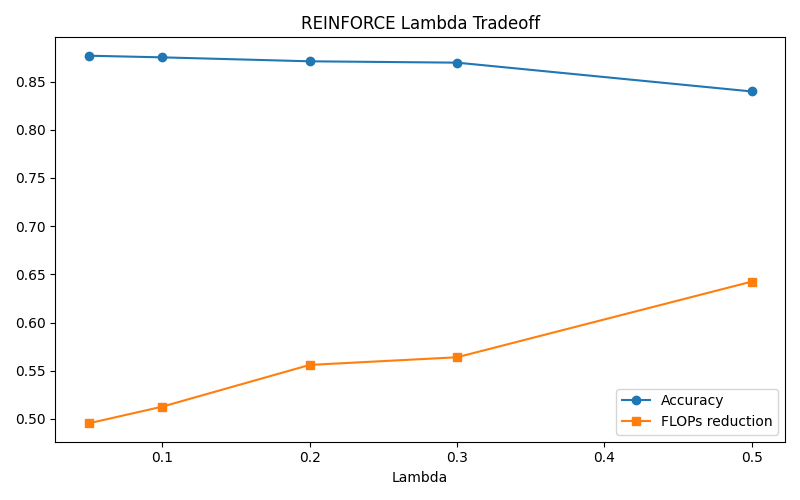
\includegraphics[width=\linewidth,height=0.145\textheight,keepaspectratio]{reinforce_lambda_tradeoff.png}
        \caption{REINFORCE lambda sweep. Lower cost weights preserve more accuracy, while larger values encourage earlier exits.}
        \label{fig:reinforce-sweep}
    \end{subfigure}
    \caption{Grouped policy-sweep figures for side-by-side comparison with the main frontier in Figure~\ref{fig:accuracy-flops}. From left to right: the fixed-threshold sweep, the supervised-controller reward-label sweep, and the REINFORCE reward sweep.}
    \label{fig:policy-sweeps}
\end{figure*}

\subsection{Ablation Studies}

Table~\ref{tab:ablation} collects representative ablation points across policy families. Together with Figures~\ref{fig:threshold-ablation}, \ref{fig:controller-sweep}, and \ref{fig:reinforce-sweep}, it highlights that the main design problem is not whether earlier exits save compute, but whether a policy can use them without sacrificing too much accuracy.

\begin{table*}[!tbp]
\centering
\caption{Representative ablation points from the source-of-truth run.}
\label{tab:ablation}
\footnotesize
\setlength{\tabcolsep}{3pt}
\renewcommand{\arraystretch}{1.05}
\begin{tabularx}{\textwidth}{@{}YccccY@{}}
\toprule
Setting & Accuracy & \makecell{FLOPs\\Red.} & Latency & \makecell{Avg.\\Exit} & Notes \\
\midrule
Fixed threshold $\tau=0.50$ & 76.05\% & 71.68\% & 0.062 ms & 1.30 & Extremely aggressive early exiting \\
Fixed threshold $\tau=0.95$ & 87.53\% & 42.73\% & 0.074 ms & 2.51 & Strong manual tradeoff point \\
Fixed threshold $\tau=0.99$ & 87.73\% & 32.83\% & 0.080 ms & 2.88 & Best fixed-threshold accuracy \\
Dynamic budget-first $0.90/0.50$ & 85.53\% & 60.41\% & 0.054 ms & 1.82 & Best dynamic compute saving among listed points \\
Supervised controller $\lambda=0.30$ & 72.52\% & 74.33\% & 0.053 ms & 1.18 & Best supervised accuracy, but poor overall frontier \\
REINFORCE $\lambda=0.05$ & 87.69\% & 49.54\% & 0.086 ms & 2.32 & Best learned-policy accuracy \\
\bottomrule
\end{tabularx}
\end{table*}

Bootstrap resampling supports cautious comparison rather than significance claims. The full baseline has a 95\% bootstrap accuracy interval of [87.66\%, 88.85\%], the best fixed-threshold policy has [87.09\%, 88.39\%], and the best REINFORCE policy has [87.00\%, 88.39\%]. These intervals overlap substantially, which is consistent with the small absolute accuracy gaps between the strongest methods.

\subsection{Additional Analysis}

The deeper metrics also support a more detailed view of routing behavior, uncertainty, and class-level errors. Figure~\ref{fig:exit-distribution} and Table~\ref{tab:exit-behavior} show that the strongest policies do not merely save compute; they do so through very different routing patterns. The dynamic accuracy-first policy collapses to the final head, the fixed-threshold policy uses exits 2 and 3 heavily while still sending 35.86\% of samples to the final head, the supervised controller exits 82.63\% of samples at the first head, and the strongest REINFORCE policy concentrates most traffic at exits 2 and 3.

\begin{figure}[!tbp]
    \centering
    
\includegraphics[width=\linewidth,height=0.23\textheight,keepaspectratio]{exit_distribution_comparison.png}
    \caption{Exit-distribution comparison for representative methods. The dynamic accuracy-first policy behaves like a full-depth classifier, the fixed-threshold policy distributes samples across intermediate and final exits, the supervised controller exits overwhelmingly at the first head, and the strongest REINFORCE policy mostly routes samples to exits 2 and 3.}
    \label{fig:exit-distribution}
\end{figure}

\begin{table*}[!tbp]
\centering
\caption{Representative exit behavior from \texttt{per\_exit\_analysis.json}. Fractions are reported over the CIFAR-10 test set, and per-exit accuracies are conditional on samples that actually leave at that exit. `N/A' indicates that no test samples exited at that branch, so the corresponding conditional accuracy is undefined rather than 0\%.}
\label{tab:exit-behavior}
\scriptsize
\setlength{\tabcolsep}{2pt}
\renewcommand{\arraystretch}{1.05}
\begin{tabularx}{\textwidth}{Y*{8}{Z}}
\toprule
Method & \makecell{Exit 1\\frac.} & \makecell{Exit 2\\frac.} & \makecell{Exit 3\\frac.} & \makecell{Final\\frac.} & \makecell{Exit 1\\acc.} & \makecell{Exit 2\\acc.} & \makecell{Exit 3\\acc.} & \makecell{Final\\acc.} \\
\midrule
Dynamic (acc.-first $0.90/0.50$) & 0.00 & 0.00 & 0.00 & 1.00 & N/A & N/A & N/A & 87.74\% \\
Fixed threshold $\tau=0.99$ & 0.0187 & 0.4403 & 0.1824 & 0.3586 & 98.40\% & 98.71\% & 96.98\% & 68.99\% \\
Supervised controller $\lambda=0.30$ & 0.8263 & 0.1661 & 0.0076 & 0.0000 & 71.87\% & 76.58\% & 53.95\% & N/A \\
REINFORCE $\lambda=0.05$ & 0.0000 & 0.6893 & 0.2987 & 0.0120 & N/A & 96.01\% & 70.97\% & 25.83\% \\
\bottomrule
\end{tabularx}
\end{table*}

Figure~\ref{fig:bootstrap-ci} and Table~\ref{tab:bootstrap-summary} summarize the bootstrap uncertainty estimates. These intervals come from deterministic prediction resampling rather than repeated training seeds, so they should be read as uncertainty estimates for the observed runs rather than evidence of formal statistical significance. Even with that limitation, the baseline, fixed-threshold, dynamic, and REINFORCE intervals overlap closely, while the supervised controller is separated well below the main frontier.

\begin{figure}[!tbp]
    \centering
    
\includegraphics[width=\linewidth,height=0.23\textheight,keepaspectratio]{bootstrap_confidence_intervals.png}
    \caption{Bootstrap 95\% confidence intervals for representative method accuracies. The baseline, fixed-threshold, dynamic, and REINFORCE methods remain tightly clustered, whereas the supervised controller is clearly separated at much lower accuracy.}
    \label{fig:bootstrap-ci}
\end{figure}

\begin{table}[!tbp]
\centering
\caption{Bootstrap uncertainty summary from \texttt{bootstrap\_statistics.json}. The intervals are resampling-based uncertainty estimates for deterministic predictions, not repeated-training confidence bounds.}
\label{tab:bootstrap-summary}
\scriptsize
\setlength{\tabcolsep}{2pt}
\renewcommand{\arraystretch}{1.05}
\resizebox{\linewidth}{!}{%
\begin{tabular}{lrrrr}
\toprule
Method & Mean acc. & Std. & 95\% CI low & 95\% CI high \\
\midrule
Baseline & 88.27\% & 0.0032 & 87.66\% & 88.85\% \\
Fixed threshold $\tau=0.99$ & 87.75\% & 0.0034 & 87.09\% & 88.39\% \\
Dynamic (acc.-first $0.90/0.50$) & 87.76\% & 0.0034 & 87.09\% & 88.40\% \\
Supervised controller $\lambda=0.30$ & 72.53\% & 0.0045 & 71.67\% & 73.43\% \\
REINFORCE $\lambda=0.05$ & 87.70\% & 0.0034 & 87.00\% & 88.39\% \\
\bottomrule
\end{tabular}}
\end{table}

Table~\ref{tab:classification-quality} makes the aggregate classification-quality story explicit using `classification\_metrics.json`. The baseline remains strongest on accuracy, macro-F1, weighted-F1, macro precision, and macro recall, while the fixed-threshold, dynamic, early-exit-final, and REINFORCE results all stay close together in the high-0.87 range. The supervised controller drops sharply on every classification-quality metric, and weighted-F1 remains very close to accuracy across all methods because CIFAR-10 is class-balanced and the evaluation uses equal class support.

\begin{table}[!tbp]
\centering
\caption{Classification-quality summary from \texttt{classification\_metrics.json}. Values are reported for the same representative methods used throughout the Results section.}
\label{tab:classification-quality}
\scriptsize
\setlength{\tabcolsep}{2pt}
\renewcommand{\arraystretch}{1.03}
\resizebox{\linewidth}{!}{%
\begin{tabular}{@{}lccccc@{}}
\toprule
Method & Acc. & Macro-F1 & W.-F1 & \makecell{Macro\\Prec.} & \makecell{Macro\\Rec.} \\
\midrule
Baseline & 88.26\% & 88.12\% & 88.12\% & 88.76\% & 88.26\% \\
Early-exit final & 87.74\% & 87.72\% & 87.72\% & 88.13\% & 87.74\% \\
Fixed $\tau=0.99$ & 87.73\% & 87.71\% & 87.71\% & 88.13\% & 87.73\% \\
Dynamic acc.-first & 87.74\% & 87.72\% & 87.72\% & 88.13\% & 87.74\% \\
Supervised $\lambda=0.30$ & 72.52\% & 72.03\% & 72.03\% & 72.86\% & 72.52\% \\
REINFORCE $\lambda=0.05$ & 87.69\% & 87.66\% & 87.66\% & 88.09\% & 87.69\% \\
\bottomrule
\end{tabular}}
\end{table}

Finally, Figure~\ref{fig:confusion-matrix} shows that the strongest threshold and REINFORCE policies largely preserve the baseline confusion structure, while the supervised controller causes broader degradation. Table~\ref{tab:classification-quality} is consistent with that picture: the small macro-F1 gap between the baseline and the strongest threshold or REINFORCE policies indicates limited aggregate quality loss, whereas the supervised controller's drop is visible both in the confusion matrix and in every aggregate classification metric. The per-class metrics sharpen that conclusion further: relative to the baseline, the supervised controller loses 38.6 points on class 2, 23.5 points on class 4, and 19.6 points on class 5, whereas the strongest REINFORCE policy stays much closer to the baseline and even improves classes 3, 6, and 8 slightly in the current test run. The dynamic accuracy-first policy looks nearly identical to the early-exit final head because it never exits early.

\begin{figure*}[!tbp]
    \centering
    
\includegraphics[width=0.84\textwidth,height=0.43\textheight,keepaspectratio]{confusion_matrix_best_methods.png}
    \caption{Confusion matrices for the baseline, early-exit final head, best fixed-threshold policy, best dynamic policy, best supervised controller, and best REINFORCE controller. The supervised controller shows the broadest degradation pattern, while fixed threshold and REINFORCE remain visually close to the baseline.}
    \label{fig:confusion-matrix}
\end{figure*}

\section{Discussion}

Three conclusions stand out. First, the early-exit backbone itself is viable: its final-head accuracy stays close to the full baseline. Second, simple thresholding is harder to beat than expected. The fixed-threshold curve is smooth, interpretable, and already delivers near-baseline accuracy with moderate compute savings. Third, learned routing is not automatically better. The supervised \texttt{best\_reward} controller exits far too early and loses too much accuracy, while REINFORCE improves the learned-policy story substantially by shifting traffic toward exits 2 and 3 instead of collapsing onto exit 1.

The dynamic-threshold family also provides a useful negative result. In the source-of-truth run, the best-accuracy dynamic policy degenerates to always using the final exit, which means the added scheduling flexibility does not translate into a better frontier than the fixed-threshold baseline. This is still informative: it suggests that the current dynamic rule and hyperparameterization are not strong enough to justify their extra complexity on \dataset{}.

The strongest learned result is REINFORCE with $\lambda_{\text{cost}} = 0.05$. It preserves accuracy within 0.57 points of the full baseline while saving 49.54\% of FLOPs. Even so, it does not clearly exceed the best fixed-threshold accuracy point, so the fairest conclusion is that REINFORCE is promising but not yet dominant in this project setting.

\section{Limitations}

The study is limited to \dataset{}, so the conclusions should not be generalized to larger datasets or deployment settings without further evidence. The latency results should also be interpreted carefully: policy latencies in the deeper run come from staged conditional execution, while the baseline latency is inherited from the reference comparison file. That makes the relative ordering useful, but it weakens any strong claim about exact absolute latency gaps.

Emissions reporting is another important limitation. The baseline and early-exit CO$_2$ values come from CodeCarbon-wrapped training runs, whereas threshold, controller, and REINFORCE CO$_2$ values are FLOPs-scaled estimates rather than direct measurements. Those values are still useful for comparing relative compute intensity, but they should not be presented as directly observed inference emissions.

Finally, the project uses one main experimental trajectory plus ablation sweeps and bootstrap analysis, not a full multi-seed benchmark across every family. The results are therefore best read as a careful empirical case study of adaptive inference behavior on \dataset{}.

\section{Conclusion}

This project evaluated when a CNN should stop computation early on \dataset{} by comparing fixed thresholds, dynamic thresholds, a supervised controller, and a REINFORCE controller on top of an early-exit \backbone{}. The main empirical message is that the early-exit backbone is competitive, fixed thresholding is a very strong baseline, and REINFORCE offers the strongest learned policy in the current evidence. The supervised \texttt{best\_reward} controller exits too aggressively, and the best-accuracy dynamic-threshold setting collapses to the final head rather than improving the frontier.

The most practical result in the current experiments is the fixed-threshold policy at $\tau = 0.99$, which retains 87.73\% accuracy while reducing FLOPs by 32.83\%. The strongest learned-policy result is REINFORCE with $\lambda_{\text{cost}} = 0.05$, which reaches 87.69\% accuracy with 49.54\% FLOPs reduction. Future work should improve latency benchmarking consistency, verify emissions under a dedicated inference setup, and test whether the same conclusions hold on larger datasets.

\section*{Acknowledgements}

I would like to express my sincere gratitude to Professor Leandro Marcolino, the course instructor, for his guidance and constructive advice throughout this project. His input contributed significantly to improving both the quality of the experimental investigation and the development of the project ideas. I also acknowledge the use of open-source tools, including Python, PyTorch, and Matplotlib, in implementing and evaluating this work. AI-assisted tools were used only to support writing clarity, LaTeX formatting, and report organization; all implementation decisions, experiments, analysis, and final claims were reviewed and verified by the author. Additional details are provided in the required statement file.
\balance
\bibliographystyle{plainnat}
\bibliography{refs}

\end{document}
